\documentclass[../../DD.tex]{subfiles}
\begin{document}
\newpage
\subsection{Group of Topic \label{sect:2.1}}

  \subsubsection{Person}
      Single \textit{Person} page represents information about the \textit{People} who works for \textit{VenTour}. 
      On the top of the page general information about the person are shown: name and surname, the role he or she plays within the company and the team he or she is part of.\\
      Below, social icons with links at social pages are reported.
      Next to the image of the team member, information about him or her are shown in three different sections (\textit{Bio, Awards, CV}) switchable thanks to relative buttons.
      At the bottom of the web page, there are some cards of the \textit{Companies} of which the person is a supervisor. If the user click on that cards, can access to the company related page.
      There is also the possibility to return at the \textit{Our Team} page by clicking on the arrow at the top of the Person page.

    \begin{figure}[!htb]
      \centering
      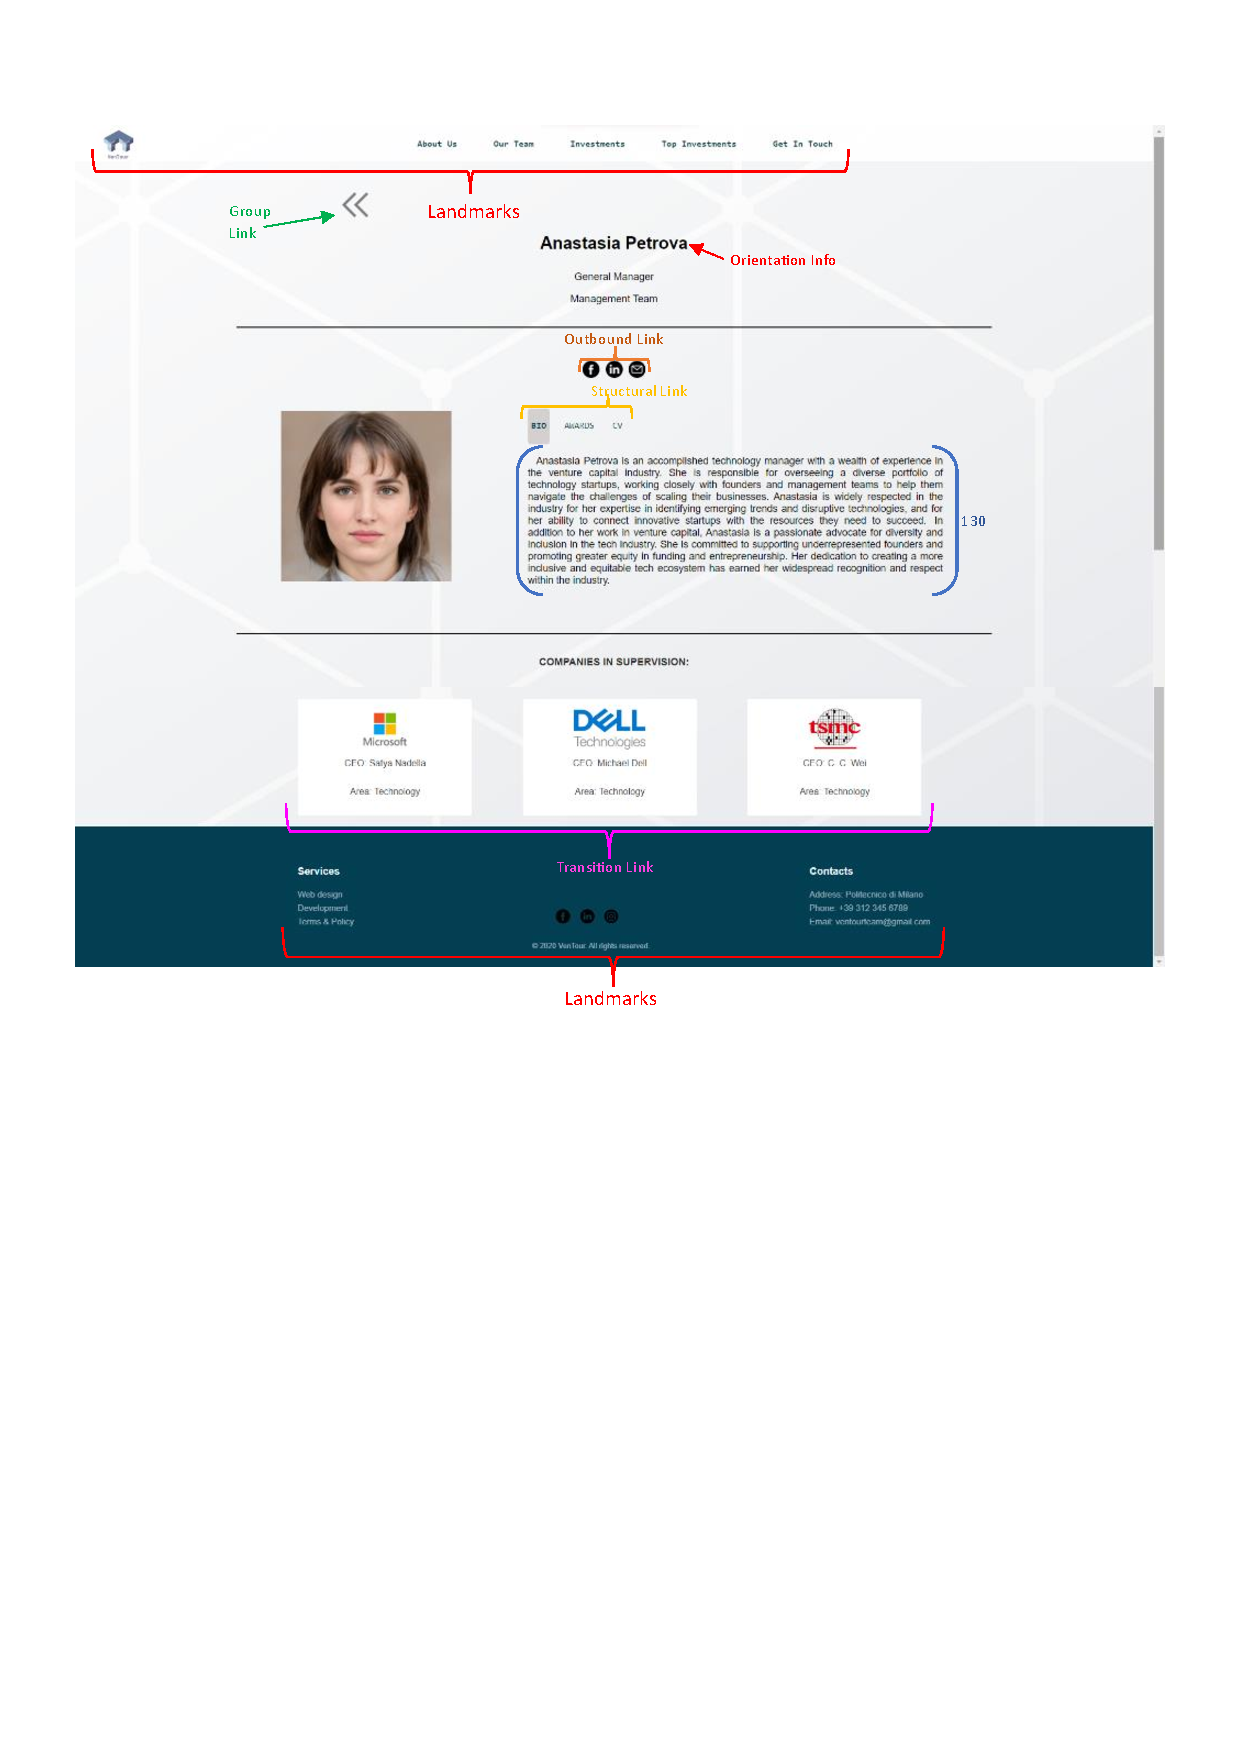
\includegraphics[width=\textwidth, trim=0 250 0 0, clip]{Images/screenshots/Person_screen.pdf} % left, bottom, right, and top 
      \caption{Person page}
      \label{fig: Person_screen}
  \end{figure}

	\subsubsection{Investment}
		Single \textit{Investment} page represents information about the \textit{Company} in which our venture company has invested on. 
  On the top of the page under the name of the company there are links to the \textit{Investment Area} at which this investment belongs to, and a link to the \textit{supervisor} of this investment, which is a member of our team. Between these links is mentioned the CEO of the company.\\The information below includes the logo of the company and a short general information about the company itself. At the end of the information there is the link to the official website of the specific company, which is an outbound link.
		\newline
		\image{\textheight}{screenshots/company scr.png}{Investment (Company) page screenshot}{Inveestment-screenshot}



  
\end{document}
